\section{Characterization of CUDA Kernels}\label{sec:characterization}
The current architectures of GPUs have a hierarchical memory management, where cores make data requests in their registers, these requests pass through caches that in some cases may be shared caches, and so on until to arrive to its global memory. When a request data of a thread increases of level in the memory hierarchy, it increases increases the communication latency. On the contrary, while higher memory level, higher  capacity of storage, see Figure~\ref{fig:PyrLatency}. 

\begin{figure}[htpb]
\centering
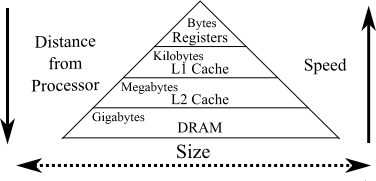
\includegraphics[scale=.75]{./images/memhierarchy.png}
\caption{Variance of the latency and capacity of storage in the memory systems}
\label{fig:PyrLatency}
\end{figure}

The performance of a function executed over a GPU depends greatly on the optimizations made in the accesses to data in the memory hierarchy. The bandwidth of the memory is optimized by grouping a set of threads, so, the threads in the group are benefited in the communication. This effect is called coalesced accesses~\citep{Wu:2013:Coalesced, Che:2011}. In Tesla architectures, the first GPGPU architecture, these coalesced accesses were by threads of a half warp, i.e. 16 threads can be coalesced to one transaction for word of size 8-bit, 16-bit, 32 bit, 64-bit or 128-bit. On Fermi, Kepler and newer architectures coalesced accesses can be done by all threads of a warp.

Since the early generations of GPUs for general purpose, GPUs have had different types of memories, which are differentiated by the type and visibility in the data. In Table~\ref{tab:memories} are presented the different types of memories existing in current GPUs. This table shows the type of operation that each memory can do. 
The constant memory is an off-chip and it can be read by all threads in a kernel, however the CPU is the only which can write on it. 
The On Chip memories are those that are inside each multiprocessors and consequently the communication latency is lower. Global memory is the main memory of the GPU, local and constant memory are just different addressing modes of the global memory. Global Memory is DRAM, on the contrary, all on-chip memory (shared memory, registers, and caches) are SRAM. 

\begin{table}[htpb]
\centering
\begin{tabular}{| l | c | c | c  |  c |} 
\hline \hline%inserts double horizontal lines
\textbf{Type} & \textit{\textbf{On Chip}}&\textbf{Cacheable}&\textbf{Operations}&\textbf{Visibility} \\ \hline
Registers&Yes&No&Read/Write&\textit{Thread}\\ \hline
Local&Not&Yes&Read/Write&\textit{Thread}\\ \hline
Shared&Yes&No&Read/Write&Block\\ \hline
Global&No&Yes&Read/Write&\textit{Kernels}\\ \hline
Constant&No&Yes&Read&\textit{Kernels}\\ \hline
Texture&No&Yes&Read/Write&\textit{Kernels}\\ \hline
\hline
\end{tabular}
\caption{Memory types of the GPUs manufactured by Nvidia}
\label{tab:memories} % is used to refer this table in the text
\end{table}

We analyzed different kernels, aiming to show which are the different optimizations that impact the performance of a GPU application. Figure~\ref{fig:BlockTunning} shows the running times of the kernel of matrix multiplication using only global memory without coalesced accesses, i.e. the kernel $MMGU$. The experiments are done varying the number of threads per block, with dimensions of $8\times{}8$, $16\times{}16$, or $32\times{}32$. Figure~\ref{fig:BlockTunning}A shows the running times, Figure~\ref{fig:BlockTunning}B the number of load transactions per request in the global memory and Figure~\ref{fig:BlockTunning}C the number of store transactions per request in the global memory. This kernel has a bad access in the global memory, for this reason it reach higher performance when the dimension of the blocks is lower.

\begin{figure}[htpb]
	\centering
    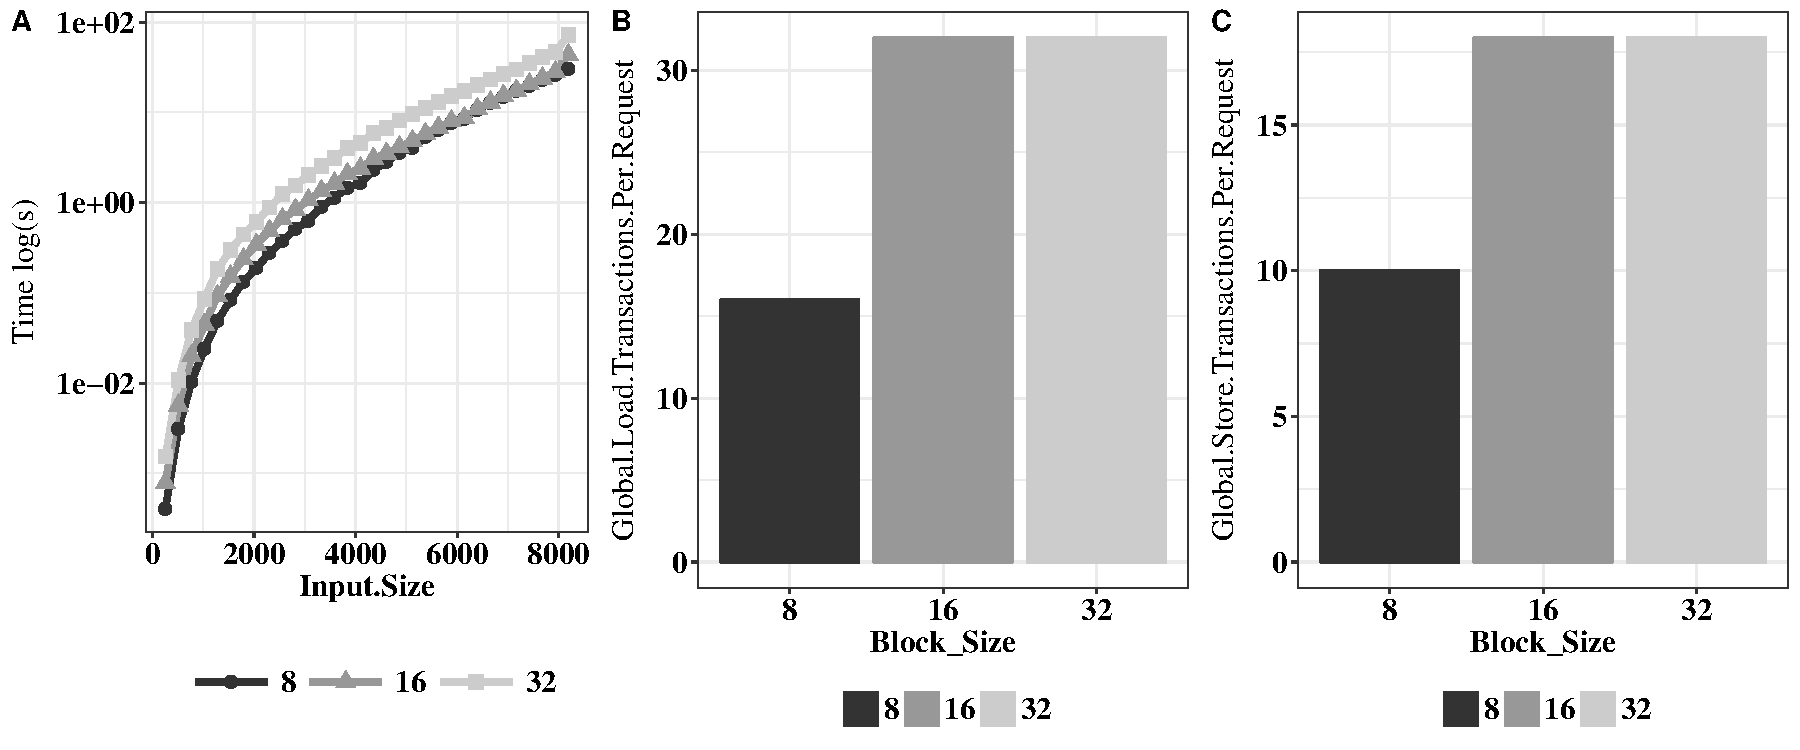
\includegraphics[scale=.5]{images/plotBlock.pdf}
    \caption{Tuning of threads per Block in MMGU on the GPU GTX-970}
    \label{fig:BlockTunning}
\end{figure}

Figure~\ref{fig:Coalesced} show the performance of two application in two different versions each one, the applications are matrix multiplication and matrix addiction, the versions  of these applications are $MMGC$ and $MMGU$; and, $MAC$ and $MAU$; respectively. The selected dimensions of threads per block in each kernel was $8\times{}8$. Each kernel change communication pattern in the global memory. Figure~\ref{fig:Coalesced}A shows the running time of the kernels $MMGC$ and $MMGU$ and Figure~\ref{fig:Coalesced}B the number of load transactions per request in the global memory. Figure~\ref{fig:Coalesced}C shows the running time of the kernels $MAC$ and $MAU$ and Figure~\ref{fig:Coalesced}D the number of load transactions per request in the global memory of two different version of the matrix addition. It is easy to perceive that when the number of transaction per request in the global memory is smaller the running time of the application improve and consequently the arithmetic throughput of the application.

\begin{figure}[htpb]
	\centering
    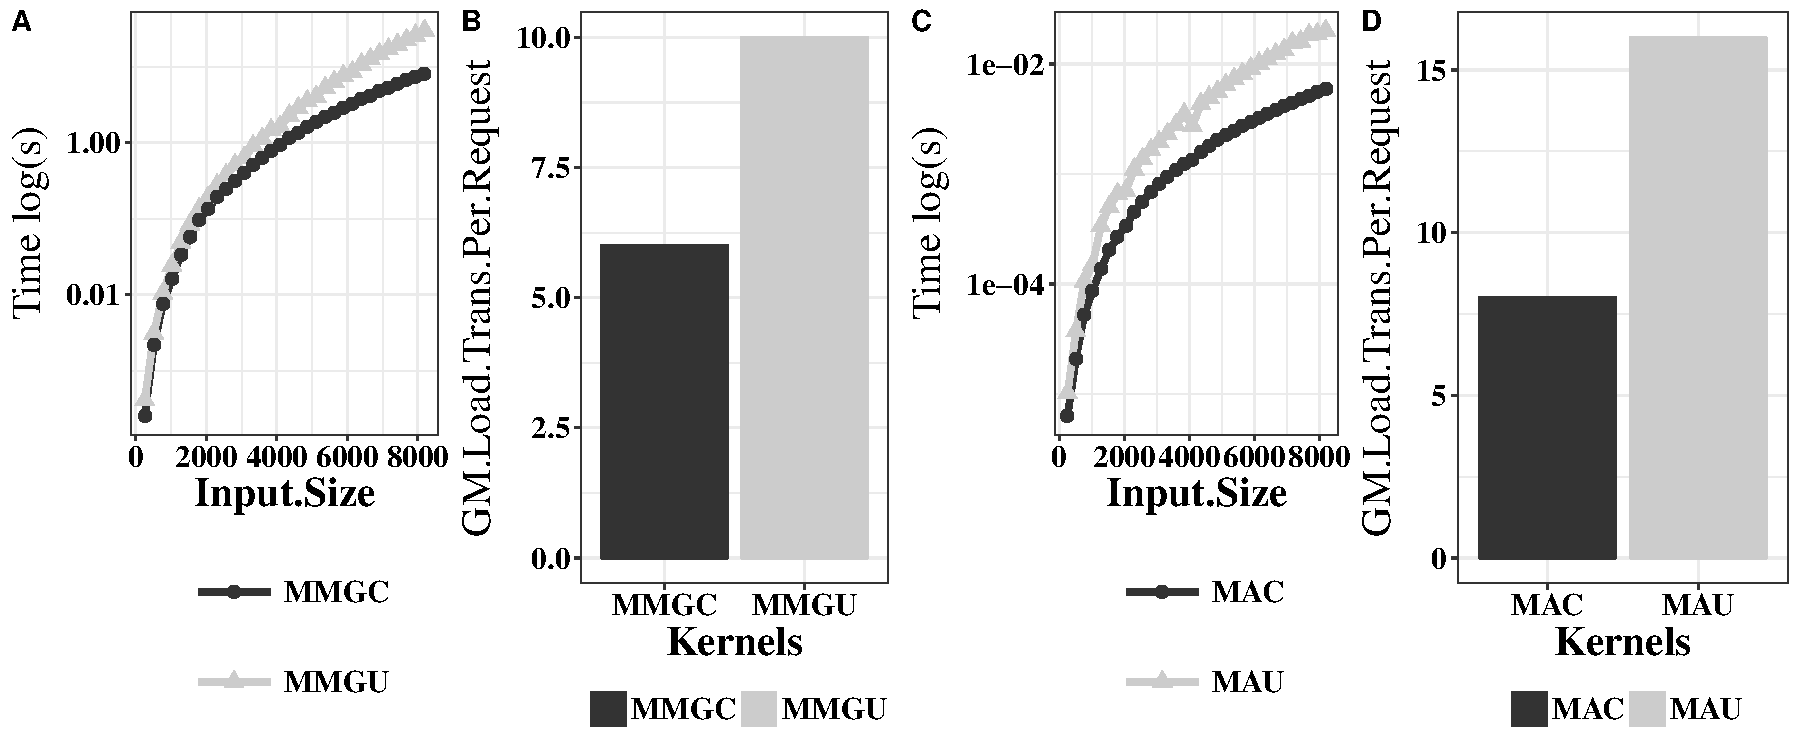
\includegraphics[scale=.5]{images/plotCoalesced.pdf}
    \caption{Coalesced accesses impact in 2 different kernels of Matrix Multiplication and Matrix Addition on the GPU GTX-970}
    \label{fig:Coalesced}
\end{figure}

Figure~\ref{fig:Shared} shows the impact of the shared memory and coalesced accesses in the 4 versions of matrix multiplication. Figure~\ref{fig:Shared}A shows the running time of the kernels $MMGU$, $MMGC$, $MMSU$ and $MMSC$; Figure~\ref{fig:Shared}B shows the throughput in the global memory and Figure~\ref{fig:Shared}C shows the number of load transactions per request in the global memory of the 4 kernels. The worst throughput in the load memory is done for the kernel $MMSU$, it means that using shared memory does not improve the throughput  in the load memory, coalesced accesses are necessary for this goal.


\begin{figure}[htpb]
	\centering
    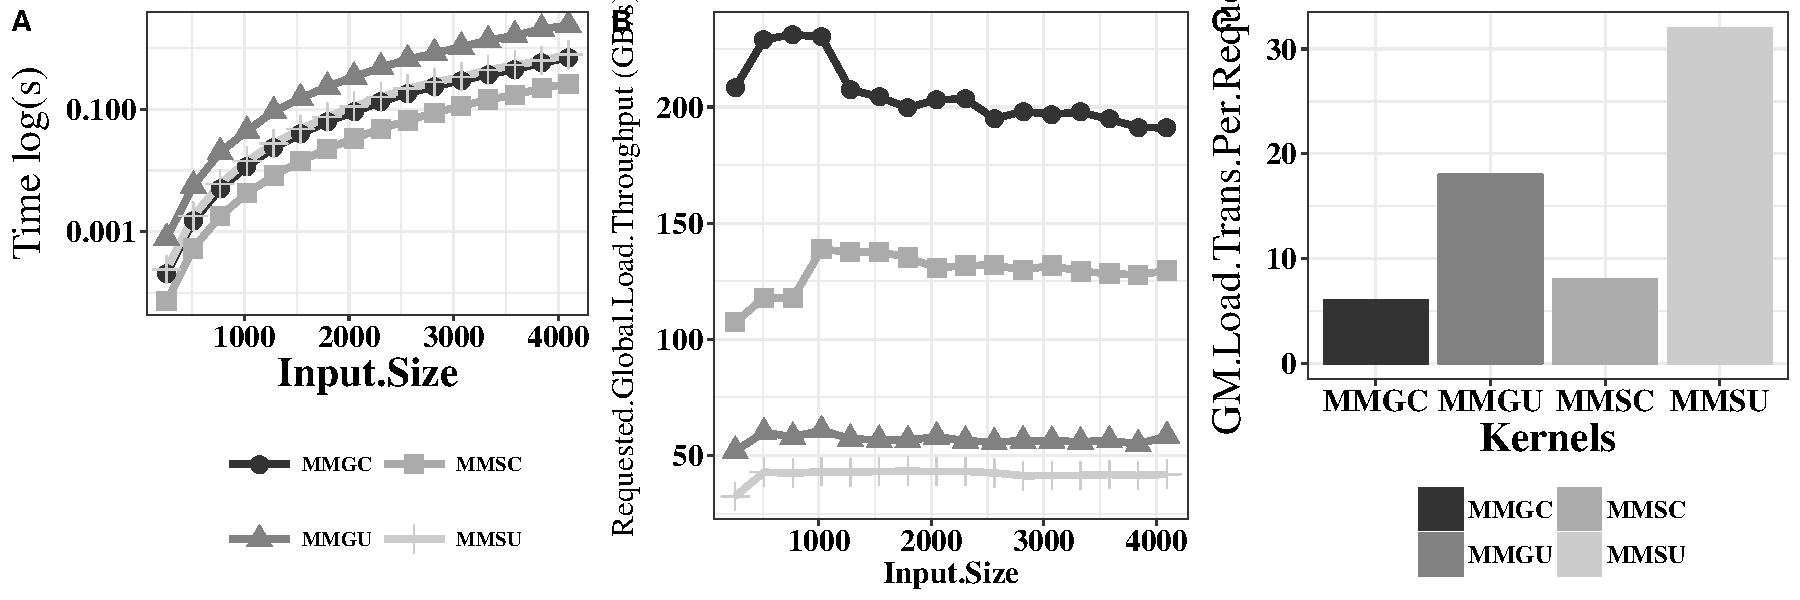
\includegraphics[scale=.5]{images/plotCoalescedShared.pdf}
    \caption{Shared memory optimizations in kernels of Matrix Multiplication on the GPU GTX-970}
    \label{fig:Shared}
\end{figure}

In ont of the work indirectly relate with this thesis, we implemented an autotuner for the CUDA compiler using the use the OpenTuner 
framework~\cite{ansel2014opentuner} and used it to search for the compilation parameters  that optimize the performance of different GPU applications.

Figure~\ref{fig:autotuning} shows the results of an implemented autotuner for the CUDA compiler using the use the OpenTuner framework~\citep{ansel2014opentuner} and used it to search for the compilation parameters that optimize the performance of GPU applications. The main result is this research was to show that it is possible to optimize code written for GPUs by automatically tuning just the parameters of the CUDA compiler.

\paragraph{The Search Space}\label{sec:parameters}

% \newcommand{\specialcell}[1]{\begin{minipage}[m]{0.52\columnwidth}\centering#1\end{minipage}}

\begin{table}[htpb]
    \centering
    \footnotesize
        \begin{tabular}{cc} 
        \toprule
        \textbf{Flag}&\textbf{Description} \\\midrule
        \texttt{no-align-double} & \specialcell{Specifies that \texttt{malign-double} should not be passed as a compiler argument on 32-bit platforms. \textbf{Step}: NVCC} \\ \midrule
        \texttt{use\_fast\_math} & \specialcell{Uses the fast math library, implies \texttt{ftz=true}, \texttt{prec-div=false}, \texttt{prec-sqrt=false} and \texttt{fmad=true}. \textbf{Step}: NVCC} \\\midrule
        \texttt{gpu-architecture} & \specialcell{Specifies the NVIDIA virtual GPU architecture for which the CUDA input files must be compiled. \textbf{Step}: NVCC \textbf{Values}: \texttt{sm\_20}, \texttt{sm\_21}, \texttt{sm\_30}, \texttt{sm\_32}, \texttt{sm\_35}, \texttt{sm\_50}, \texttt{sm\_52}} \\\midrule
        \texttt{relocatable-device-code} & \specialcell{Enables the generation of relocatable device code. If disabled, executable device code is generated. Relocatable device code must be linked before it can be executed. \textbf{Step}: NVCC} \\\midrule
        \texttt{ftz} & \specialcell{Controls single-precision denormals support. \texttt{ftz=true} flushes denormal values to zero and \texttt{ftz=false} preserves denormal values. \textbf{Step}: NVCC} \\\midrule
        \texttt{prec-div} & \specialcell{Controls single-precision floating-point division and reciprocals. \texttt{prec-div=true} enables the IEEE round-to-nearest mode and \texttt{prec-div=false} enables the fast approximation mode. \textbf{Step}: NVCC} \\\midrule
        \texttt{prec-sqrt} & \specialcell{Controls single-precision floating-point squre root. \texttt{prec-sqrt=true} enables the IEEE round-to-nearest mode and \texttt{prec-sqrt=false} enables the fast approximation mode. \textbf{Step}: NVCC} \\\midrule
        \texttt{def-load-cache} & \specialcell{Default cache modifier on global/generic load. \textbf{Step}: PTX \textbf{Values}: \texttt{ca}, \texttt{cg}, \texttt{cv}, \texttt{cs}} \\\midrule
        \texttt{opt-level} & \specialcell{Specifies high-level optimizations. \textbf{Step}: PTX \textbf{Values}: \texttt{0 - 3}} \\\midrule
        \texttt{fmad} & \specialcell{Enables the contraction of floating-point multiplies and adds/subtracts into floating-point multiply-add operations (FMAD, FFMA, or DFMA). \textbf{Step}: PTX} \\\midrule
        \texttt{allow-expensive-optimizations} & \specialcell{Enables the compiler to perform expensive optimizations using maximum available resources (memory and compile-time). If unspecified, default behavior is to enable this feature for optimization level $\geqslant$O2. \textbf{Step}: PTX} \\\midrule
        \texttt{maxrregcount} & \specialcell{Specifies the maximum number of registers that GPU functions can use. \textbf{Step}: PTX \textbf{Values}: \texttt{16 - 64}} \\\midrule
        \texttt{preserve-relocs} & \specialcell{Makes the \texttt{PTX} assembler generate relocatable references for variables and preserve relocations generated for them in the linked executable. \textbf{Step}: NVLINK} \\\midrule
        \end{tabular}
    \caption{Description of flags in the search space}
    \label{tab:flags} 
\end{table}

Table~\ref{tab:flags} details the subset of the CUDA configuration
parameters used in the experiments~\footnote{Adapted from: http://docs.nvidia.com/cuda/cuda-compiler-driver-nvcc [Accessed on 20 February 2018]}.
The parameters target different compilation steps: the \emph{PTX} optimizing assembler;
the \emph{NVLINK} linker; and the \emph{NVCC} compiler.  We compared the
performance of programs generated by tuned parameters with the
standard compiler optimizations, namely \texttt{--opt-level=0,1,2,3}. 
Different \texttt{--opt-level}s could also be selected during tuning. 
We did not use compiler options that target the host linker or the library manager 
since they do not affect performance.
The size of the search space defined by all possible combinations
of the flags in Table~\ref{tab:flags} is in the order of $10^{6}$ making
hand-optimization or exhaustive searches very time consuming.

Figure~\ref{fig:autotuning} show the results of the application matrix multiplication with the 4 different version used in this work. We can see that optimizations can be done by compiler parameters, and these compiler parameters can impact the speedup of GPU application in up $4x$, this work has been done by~\cite{bruel:2017:CCPE}.

\begin{figure}[htpb]
	\centering
    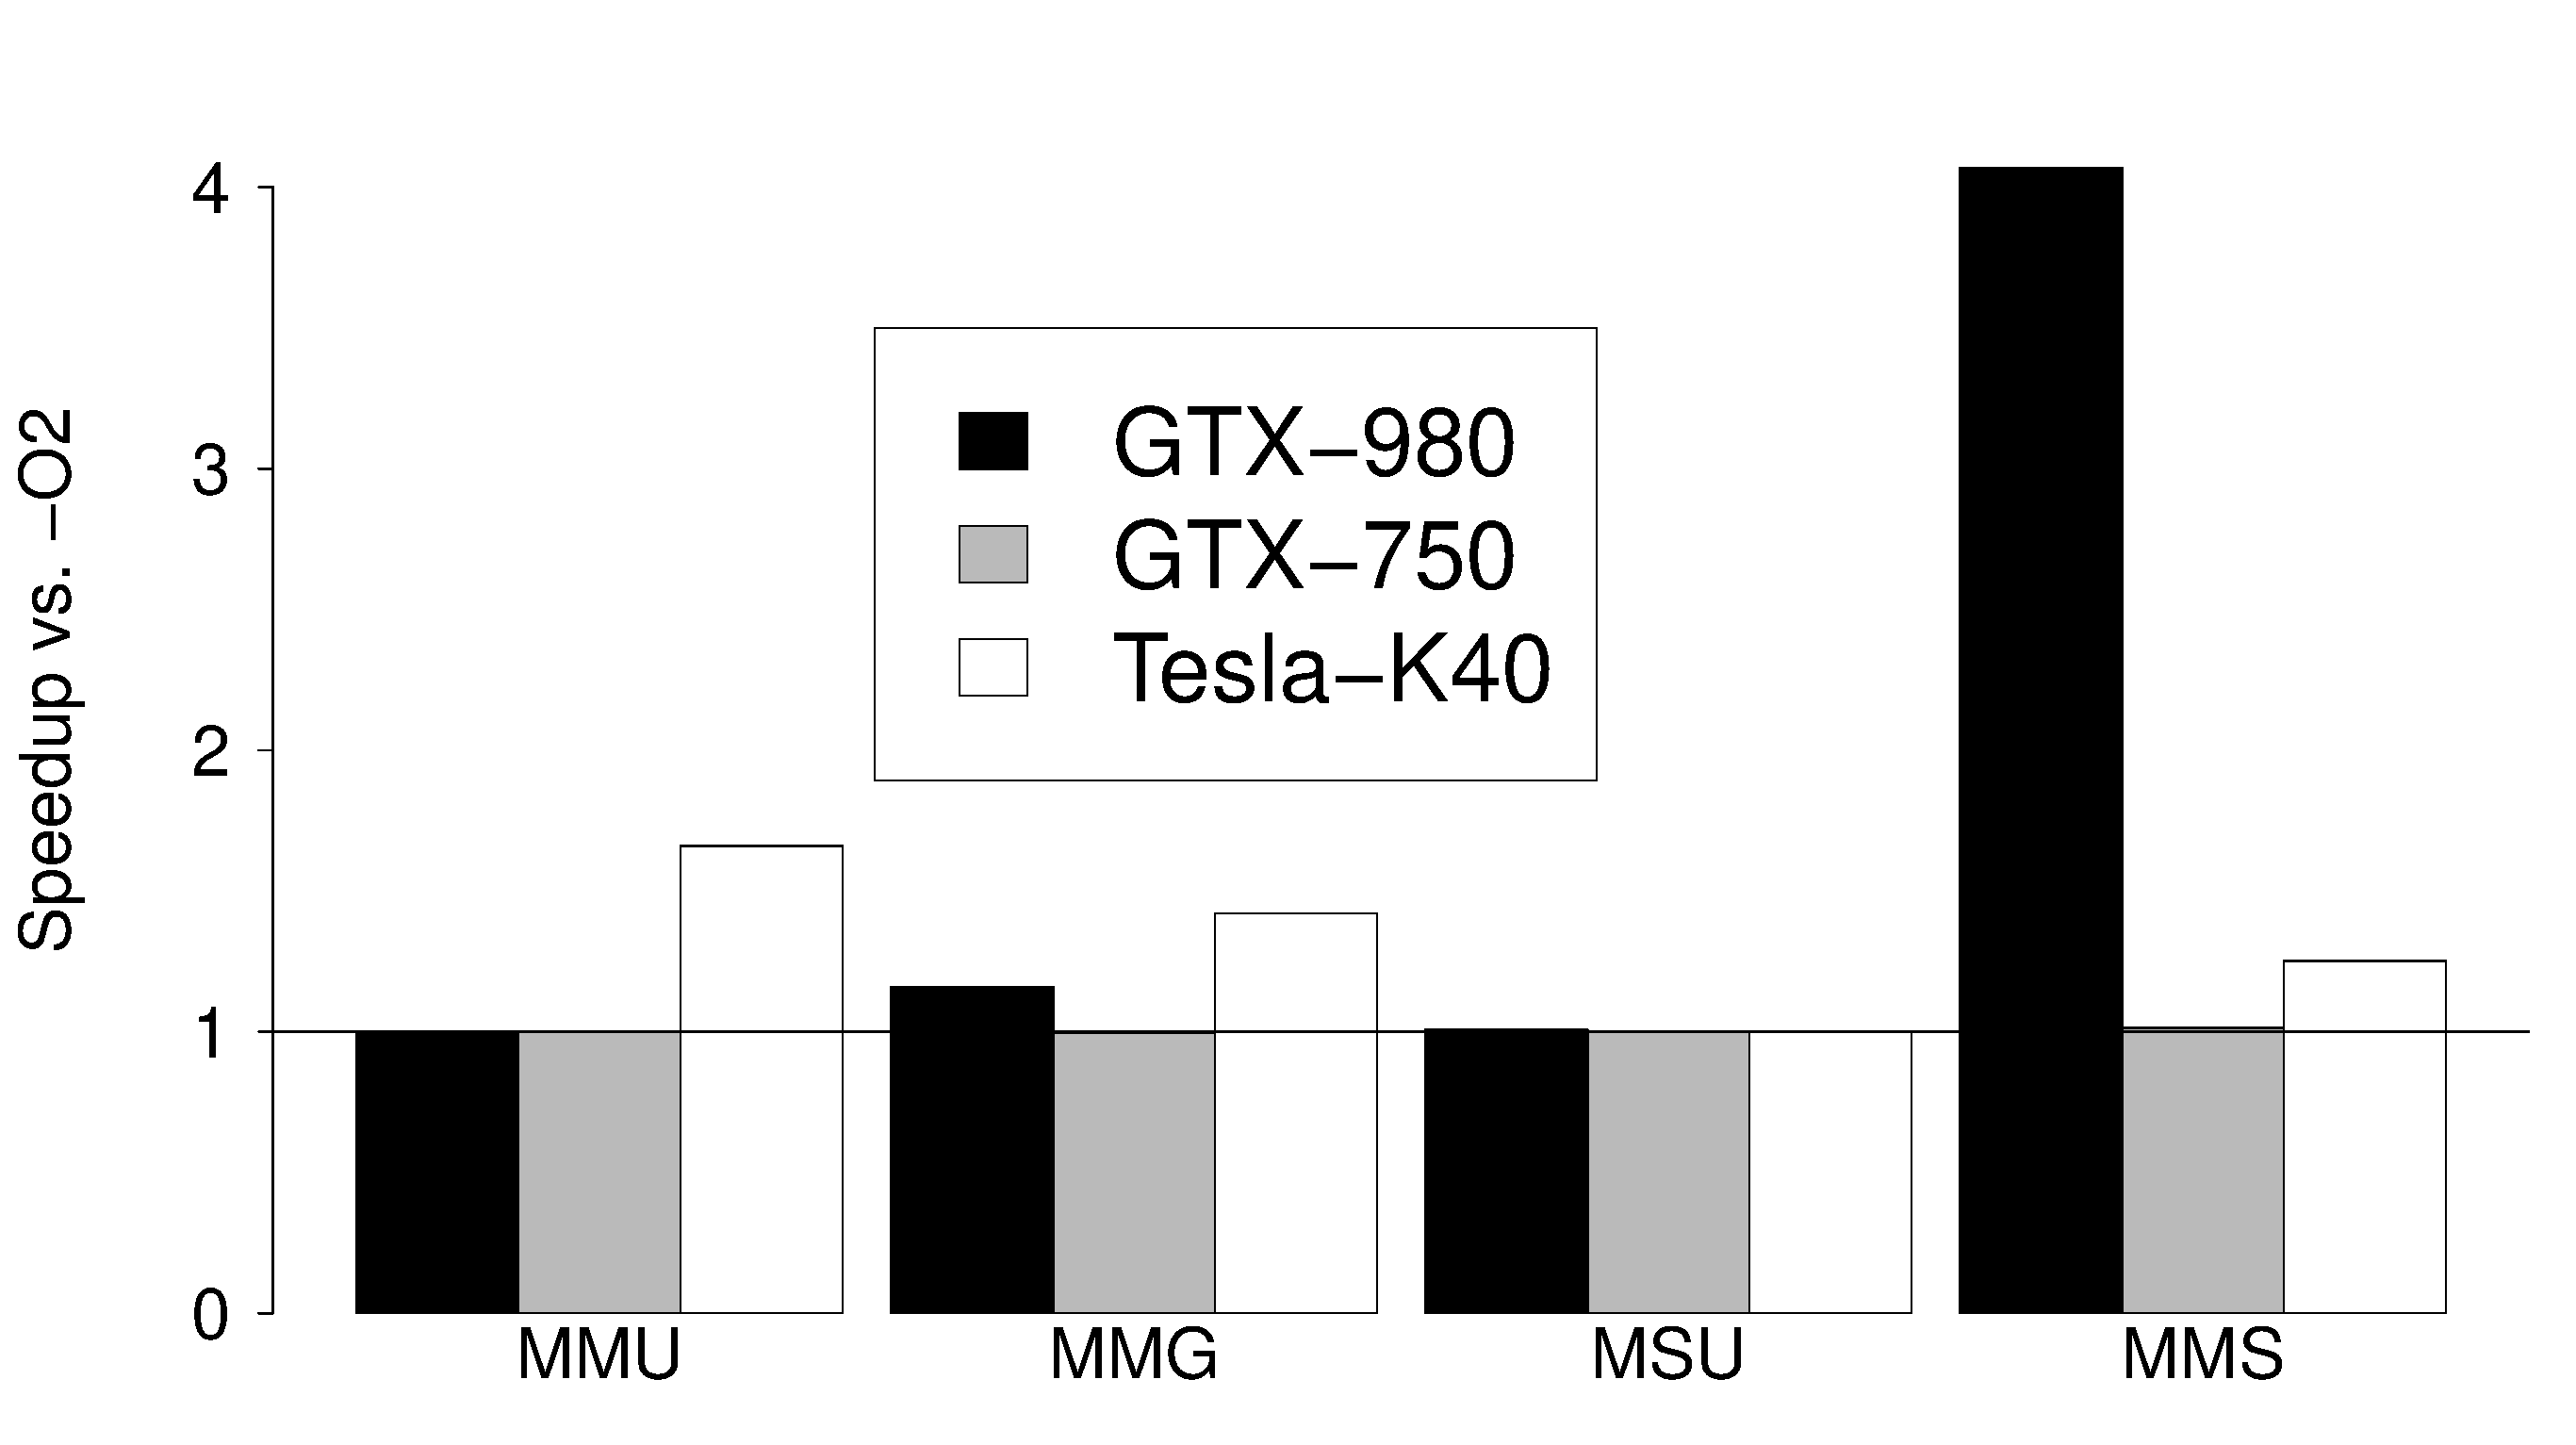
\includegraphics[scale=.2]{images/MatrixSummary.eps}
    \caption{Summary of the speedups achieved versus \emph{-O2} in matrix multiplication versions}
    \label{fig:autotuning}
\end{figure}